\documentclass{IEEEtran}

\usepackage{amsmath}
\usepackage{amsfonts}
\usepackage{amssymb}
\usepackage{blindtext}
\usepackage{graphicx}

\graphicspath{ {./images/} }

\title{Circular ISAR Work}

\author{Josiah W. Smith}


\begin{document}
	
\maketitle
	
\begin{abstract}
	Circular inverse synthetic aperture radar (CISAR) methods for near-field image reconstruction using wideband FMCW radar transceivers and wide-angle scanning. In this setup, the target scene is rotated by an angle $\theta$ and observed by the radar at various time instances.
\end{abstract}

\section{Efficient Terahertz Wide-Angle NUFFT-Based Inverse
	Synthetic Aperture Imaging Considering
	Spherical Wavefront by J. Gao}

\subsection{Math}

For the basic near-field cylindrical setup, the return signal can be modeled by equation (1).

\begin{gather}
s(\theta,k) = \iint \frac{p(x,z)}{R^2}e^{j2kR}dxdz \\
R = \sqrt{(R_0 cos\theta - x)^2 + (R_0 sin\theta - z)^2}
\end{gather}
Where $R_0$ is the radial distance from the center of the rotator to the radar transceiver.

The algorithm for recovering the reflectivity function of the target scene is described by the following derivation.

First, the exponential term in equation (1) can be approximated by:

\begin{multline}
e^{j2k\sqrt{(R_0 cos\theta - x)^2 + (R_0 sin\theta - z)^2}} \approx \\ \int_{-\pi}^{\pi} e^{j2k(cos\alpha(R_0cos\theta-x)+sin\alpha(R_0sin\theta - z))} d\alpha
\end{multline}

Substituting into equation (1) neglecting amplitude terms.

\begin{multline}
s(\theta,k) = \iint p(x,z) \\ 
\times \int_{-\pi}^{\pi} e^{j2k(cos\alpha(R_0cos\theta-x)+sin\alpha(R_0sin\theta - z))} d\alpha dx dz
\end{multline}
\begin{multline}
s(\theta,k) = \int_{-\pi}^{\pi} \iint p(x,z) e^{-j2k(xcos\alpha+zsin\alpha)}dxdz \\
\times e^{j2kR_0cos(\theta-\alpha)}d\alpha
\end{multline}

Defining the Fourier relation:

\begin{equation}
p(\alpha,k) \triangleq \iint p(x,z) e^{-j2k(xcos\alpha+zsin\alpha)}dxdz
\end{equation}

Now

\begin{equation}
s(\theta,k) = \int_{-\pi}^{\pi} p(\alpha,k) e^{j2kR_0cos(\theta-\alpha)}d\alpha
\end{equation}

It is obvious that equation (7) represents a circular convolution with respect to $\theta$, denoted by $\circledast_{\theta}$.

\begin{gather}
h(\theta,k) = e^{j2kR_0cos\theta}\\
s(\theta,k) = p(\theta,k) \circledast_{\theta} h(\theta,k)
\end{gather}

Taking the Fourier transform on both sides of equation (9) allows for multiplication in the Fourier domain to replace convolution spatial angular. Note that $\theta$ and $\Theta$ are conjugate variables of the Fourier transform.

\begin{gather}
S(\Theta,k) = P(\Theta,k)H(\Theta,k) \\
P(\Theta,k) = S(\Theta,k)H^*(\Theta,k) \\
p(\theta,k) = IFT_{1D}^{(\Theta)}\left[ S(\Theta,k)H^*(\Theta,k) \right]
\end{gather}
Where $S(\Theta,k) \triangleq FT_{1D}^{(\theta)}[s(\theta,k)]$, the Fourier transform of the received echo data with respect to $\theta$.

By the Fourier relation in equation (6), $p(x,z)$ can be recovered from $p(\theta,k)$ by:

\begin{equation}
p(x,z) = \iint p(\theta,k) e^{j2k(xcos\theta+zsin\theta)}d\theta dk
\end{equation}

Equation (13) can be viewed as a 2D inverse Fourier transform across a non-uniformly sampled domain. Using non-uniform fast Fourier transform (NUFFT) toolboxes, this integral can be calculated efficiently. 

\section{Extension to 3D Case (D. Sheen's Patent)}

Similarly, the return signal from a 2D scanner as shown in Figure 1 can be modeled by equation (14).

\begin{figure}[h]
	\centering
	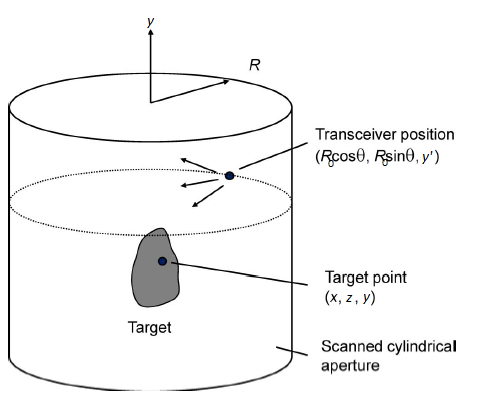
\includegraphics[scale = 0.5]{D Sheen Cylindrical Coordinate System.png}
	\centering
	\caption{2D Scanner Coordinate System}
	\label{fig:coordSys2D}
\end{figure}

\begin{gather}
s(\theta,k,y') = \iint \frac{p(x,z,y)}{R^2}e^{j2kR}dxdzdy \\
R = \sqrt{(R_0 cos\theta - x)^2 + (R_0 sin\theta - z)^2 + (y - y')^2}
\end{gather}

The exponential term in equation (14) can be decomposed using the method of stationary phase (MSP).

\begin{multline}
e^{j2k\sqrt{(R_0 cos\theta - x)^2 + (R_0 sin\theta - z)^2 + (y - y')^2}} \approx \\ \iint e^{j2k_r(cos\alpha(R_0cos\theta-x)+sin\alpha(R_0sin\theta - z)) + jk_{y'}(y - y')} d\alpha dk_{y'}
\end{multline}

Defining $k_r$ as the wavenumber in the x-z plane as:

\begin{equation}
k_r = \sqrt{k_x^2 + k_z^2} = \sqrt{4k^2 - k_{y'}^2}
\end{equation}

Where $k_{y'} \in [-2k,2k]$ and $\alpha \in [-\pi/2,\pi/2]$. IMPORTANT: Notice the difference here between Gao's paper using $k$ and Sheen's paper using $k_r$.

Ignoring the amplitude terms, equation (16) is substituted into equation (14) to yielding:

\begin{multline}
	s(\theta,k,y') = \iint_{-\pi/2}^{\pi/2} e^{j2k_r cos(\theta-\alpha)} \\ \times \left[\iiint p(x,z,y) e^{-j2k_r(xcos\alpha + zsin\alpha)-jk_{y'}y}dxdzdy\right] \\ \times e^{jk_{y'}y'}d\alpha dk_{y'}
\end{multline}

Defining the Fourier relationship:
\begin{equation}
	p(\alpha,k,k_{y'}) = \iiint p(x,z,y) e^{-j2k_r(xcos\alpha + zsin\alpha)-jk_{y'}y}dxdzdy
\end{equation}

Equation (18) can be modified as the following. Notice the exponential kernel at the end represents an inverse Fourier transform with respect to $y'$ and thus a forward Fourier transform is taken on both sides, to produce equation (22). Also, the distinction between the primed and unprimed coordinate systems is dropped for equation (22) and onward.
\begin{gather}
	s(\theta,k,y') = \iint_{-\pi/2}^{\pi/2} e^{j2k_r cos(\theta-\alpha)} p(\alpha,k,k_{y'})  e^{jk_{y'}y'}d\alpha dk_{y'} \\
	S(\theta,k,k_y) = FT_{1D}^{(y')}[s(\theta,k,y')] \\
	S(\theta,k,k_y) = \int_{-\pi/2}^{\pi/2} e^{j2k_r cos(\theta-\alpha)} p(\alpha,k,k_{y'})d\alpha 
\end{gather}

Equation (22) can be viewed as a circular convolution in the $\theta$ domain, denoted by $\circledast_{\theta}$. Defining:

\begin{gather}
	g(\theta,k,k_y) \triangleq e^{j2k_rR_0cos\theta} \\
	S(\theta,k,k_y) = p(\theta,k,k_y) \circledast_{\theta} g(\theta,k,k_y)
\end{gather}

Utilizing the Fourier relationship between convolution and multiplication:

\begin{gather}
	S(\Theta,k,k_y) = FT_{2D}^{(\theta,y)}[s(\theta,k,y)] \\
	P(\Theta,k,k_y) = FT_{1D}^{(\theta)}[p(\theta,k,k_y)] \\
	G(\Theta,k,k_y) = FT_{1D}^{(\theta)}[g(\theta,k,k_y)] \\
	S(\Theta,k,k_y) = P(\Theta,k,k_y) G(\Theta,k,k_y)
\end{gather}

Now $P(\Theta,k,k_y)$ can be recovered by either deconvolution:

\begin{gather}
	P(\Theta,k,k_y) = \frac{S(\Theta,k,k_y)}{G(\Theta,k,k_y)} \\
	P(\Theta,k,k_y) = S(\Theta,k,k_y)G^*(\Theta,k,k_y)
\end{gather}

Or for $\Theta <<2k_rR_0$, using the definition of the Hankel function of the first kind $\Theta$ order and its asymptotic form:

\begin{gather}
	G(\Theta,k,k_y) \approx e^{j\sqrt{4k_r^2R_0-\Theta^2}} \\
	P(\Theta,k,k_y) = S(\Theta,k,k_y)e^{-j\sqrt{4k_r^2R_0-\Theta^2}}
\end{gather}

Where $(\bullet)^*$ is the complex conjugate operation.

Now $p(\theta,k,k_y)$ can be recovered by:

\begin{equation}
	p(\theta,k,k_y) = IFT_{1D}^{(\Theta)}[P(\Theta,k,k_y)]
\end{equation}
Using equation (29), (30), or (32) to compute $P(\Theta,k,k_y)$.
And $p(x,z,y)$ can be computed by either (34) or (36).

\begin{gather}
	p(x,z,y) = \iiint p(\theta,k,k_y) e^{j2k_r(xcos\theta+zsin\theta) + jk_y y}d\theta dk dk_y \\
	p(\theta,k,y) = IFT_{1D}^{(k_y)}[p(\theta,k,k_y)] \\
	p(x,z,y) = \iint p(\theta,k,y) e^{j2k_r(xcos\theta+zsin\theta)} d\theta dk
\end{gather}

Equations (34) and (36) can both be viewed as inverse Fourier transforms across non-uniformly sampled data. Using non-uniform fast Fourier transform (NUFFT) toolboxes, these integrals can be calculated efficiently.

Alternately, $p(\theta,k,k_y)$ can be directly interpolated to $P(k_x,k_z,k_y)$ by the following relations and equation (17):

\begin{gather}
	k = \frac{1}{2} \sqrt{k_x^2 + k_z^2 + k_y^2} \\
	\theta = tan^{-1}\left(\frac{k_z}{k_x}\right) \\
	k_x = 2k_r cos\theta \\
	k_z = 2k_r sin\theta
\end{gather}

Then
\begin{equation}
	p(x,z,y) = IFT_{3D}^{(x,z,y)}[P(k_x,k_z,k_y)]
\end{equation}

\end{document}